\documentclass[10pt,twoside,a4paper]{article}
\usepackage[utf8]{inputenc}

\usepackage{graphicx}
\usepackage{amsmath}
\usepackage{amsfonts}
\usepackage{amssymb}
\usepackage{siunitx}
\usepackage{multicol}
\usepackage{braket}
\usepackage{parskip}
\usepackage[fontsize=6pt]{scrextend}
\usepackage[top=0.5cm, left=0.5cm, right=0.5cm, bottom=0.5cm]{geometry}

\DeclareSIUnit\fm{\femto\meter}
\DeclareSIUnit\eVpercSQ{\eV\per\clight\squared}

\newcommand{\Vek}[2]{\left(\begin{array}{c}#1\\#2\end{array}\right)}

\begin{document}
\begin{multicols*}{3}
Atomdurchmesser: $10^{-10}$\si{\meter}   Kerndurchmesser: $10^{-14}$\si{\meter}    Durchmesser Nukleon: $10^{-15}$\si{\meter}

Gesamtenergie: $E = \sqrt{m_0^2 c^4 + p^2 c^2}$, LHC: \SI{14e12}{\eV}

Elektrondrift: \SI{1}{\milli\second} $\sim$ \SI{5}{\cm}, Flugstrecke relativistisches Teilchen: \SI{1}{\nano\second} $\sim$ \SI{30}{\cm}

\textbf{relative Stärke Kräfte}: Schwerkraft $10^{-41}$, schwache WW (Quarks, Leptonen; wirkt auf Flavor): $10^{-4}$, EM WW: $1$, starke WW (Quarks, Gluonen, wirkt auf Farbladung): $60$

\textbf{Reichweite virtuelles Teilchen}: Unschärfe: $\Delta E \Delta t > \frac{\hbar}{2} \Rightarrow \Delta E \Delta t \approx mc^2 \Delta t > \frac{\hbar}{2} \Rightarrow \text{Reichweite} \approx c \Delta t > \frac{\hbar}{2mc}$ \\
EM WW (Photon): $m = 0 \Rightarrow \text{Reichweite} = \infty$ \\
schwache WW: $m_W = \SI[per-mode=symbol,per-symbol=/]{80}{\giga\eVpercSQ}, m_{Z_0} = \SI[per-mode=symbol,per-symbol=/]{91}{\giga\eVpercSQ} \Rightarrow \text{Reichweite} = \SI{0.001}{\fm}$  \\
starke WW: Gluonen mit Selbst-WW, Reichweite $\sim \SI{0.5}{\fm}$ \\
Starke Kraft: $m_{Pion} = \SI[per-mode=symbol,per-symbol=/]{140}{\mega\eVpercSQ} \Rightarrow \text{Reichweite} \sim \SI{1}{\fm}$

\textbf{Auflösung} Objekt mit Radius $R$ mit Impuls $p$: Unschärfe: $p \cdot R > \frac{\hbar}{2}$, $\Delta p_{max} = 2p \Rightarrow \Delta p_{max} \cdot R > \hbar$

\ \\
$E = \sqrt{m_0^2 c^4 + p^2 c^2}$, $P = \Vek{E/c}{\vec{p}}$, $E = E_0 + E_{kin}$, $E_0 = m_0 c^2$, $E = \gamma m_0 c^2$, $\vec{p} = \gamma m_0 \vec{v}$, $\gamma = \frac{1}{\sqrt{1 - \beta^2}}$, $\beta = \frac{v}{c}$ \\
\textbf{Invariante Masse}: $P^2 = \frac{E^2}{c^2} - \vec{p}^2 = m^2_0 c^2$ \\
\textbf{Schwerpunktsenergie $\sqrt{S}$}: nutzbare Energie in der Reaktion; invariant unter Lorenzt-Trafo; $S = (P_1 + P_2 + ...)^2$  \\
Stoßprozess: Summe der Viererimpuls bleibt erhalten

\textbf{Lorentz-Trafo}: Koordsyst. Strich bewegt sich mit Geschw. $v$ gegenüber ungestrichenem Koordsyst. in z-Richtung \\
$P' = \Vek{E'/c}{\vec{p'}}$, $P = \Vek{E/c}{\vec{p}}$ \\
$p'_x = p_x$, $p'_y = p_y$, $p'_z = \gamma p_z - \beta \gamma \frac{E}{c}$, $\frac{E'}{c} = - \beta \gamma p_z + \gamma \frac{E}{c}$

\ \\
Strahlfluss: $J = n_a \cdot v_a = \frac{\dot{N_a}}{F}$ mit $n_a$ Teilchendichte, $N_a$ Teilchen im Strahl, $F$ Querschnittsfläche Strahl \\
Luminosität: $L = J \cdot N_b$ mit $N_b$ Teilchen im Target \\
Reaktionsrate: $R = L \cdot \sigma_r$, mit $\sigma_r$ Reaktionsquerschnitt: $\sigma_r = \int \frac{d\sigma}{d\Omega} \,d\Omega$  \\
WK Wechselwirkung Strahlteilchen + Target: \\
$P = \frac{\sigma_{\text{tot}} N_{b}}{F}$, $\frac{N_{b}}{F} = n_{b} d$ mit Dicke $d$ des Targets und $N_b$ der Anzahl der Teilchen im Target mit Fläche $F$ \\
\textbf{Fermis goldene Regel}: $\sigma_{i \rightarrow f} = \frac{R}{L} = \frac{2 \pi}{\hbar v_a} \left| \mathcal{M}_{fi} \right| ^2 \cdot \rho \left( E_f \right) \cdot V$ mit $V = \frac{N_a}{n_a}$, $\rho \left( E_f \right) = \frac{dn \left( E_f \right)}{dE_f} = \frac{V \cdot 4 \pi p'^2}{v' \cdot (2 \pi \hbar)^3}$ Dichte der Endzustände, $\mathcal{M}_{fi} = \braket{\psi_f|\mathcal{H}_{WW}|\psi_i}$

\ \\
\textbf{Kosmische Strahlung}: Energien bis zu $10^{21} \si{\eV}$ \\
Primärstrahlung: $85\%$ Protonen, $14\%$ $\alpha$-Teilchen, $1\%$ schwere Kerne; Supernovae, Sonnenwind \\
Sekundärstrahlung: Erzeugung von Myonen ($> 95\%$), Protonen, Pionen (Promille-Bereich) $\Rightarrow$ Entdeckung Pion

\ \\
Elektrostatische Beschleuniger: $E_{kin} = q U$ \\
\textbf{Tandem van der Graaff}: 1-fach negativ geladenes Ion beschleunigen $\Rightarrow$ n+1 $e^-$ strippen $\Rightarrow$ n-fach positives Ion beschleunigen $\Rightarrow$ Gesamtenergie: $E_{kin} = (n+1) \cdot e U$ \\
Beschleunigungsspannung MLL: $\approx \SI{14}{\mega\V}$

\textbf{Fokussierung}: gekreuzte Quadrupolmagnete, da ein Magnet nur in eine Richtung fokussiert, aber in die andere defokussiert

\textbf{Betatron}: Nur für $e^-$. Teilchen werden durch Magnetfeld auf Bahn gehalten. Beschleunigung erfolgt durch zweites zeitlich veränderliches Magnetfeld (Induktion) \\
$F_L = q v B_H$, $v = \omega r$, $F_z = \frac{m v^2}{r}$ \\
Im GG: $F_L = F_z$ $\Rightarrow$ $p = m v = \gamma m_0 v = q B_H r$ \\
Umlaufdauer: $T = \frac{2 \pi r}{v} = \frac{2 \pi \gamma m_0}{q B_H}$ \\
Frequenz: $\omega = \frac{2 \pi}{T} = \frac{q B}{\gamma m_0}$, Zyklotronfrequenz: $\omega = \frac{e B}{m}$ \\
Beschleunigung: $E_B$ das vom zeitl. veränderl. Magnetfeld $B$ erzeugte elektr. Feld \\
$U_{ind} = \int E_B \,ds = E_{B,\phi} \cdot 2 \pi R_0 = - \frac{d}{dt} \int B \,dA = - \dot{\Phi}$ \\
$\frac{d}{dt} p = F = e E_{B,\phi} = \frac{e \dot{\Phi}}{2 \pi R_0} = \frac{d}{dt} e B_H r = e \dot{B_H} r +  e B_H \dot{r} = e \dot{B_H} R_0$ \\
$\Rightarrow$ Haltefeld $B_H$ steigt proportional zum Elektronenimpuls an \\
$R_0^2 \dot{B_H}(R_0) = E_{B,\phi} \cdot R_0 = \frac{d}{dt} \int_{0}^{R_0} R \cdot B(R) \,dR = \frac{d}{dt} \bar{B} \cdot \frac{R_0^2}{2}$ \\
$\Rightarrow$ $B_H(r = R_0) = \frac{1}{2} \bar{B}(r = R_0)$ \\
Stabilisierung: $F_L$ muss mit wachsendem $R$ schwächer abfallen als $F_z$ $\Rightarrow$ $B_H \sim R^{-n}$, $0 < n < 1$, $n = - \frac{R}{B_{H,z}} \frac{dB_{H,z}}{dR}$ \\
Rückstellkraft erzeugt Betatron-Schwingung: $\omega_r = \sqrt{1-n} \; \omega_0$, $\omega_z = \sqrt{n} \; \omega_0$, $\omega_r \neq \omega_z \neq \omega_0$ \\
$E_{max} \approx 20 - 300 \si{\mega\eV}$

\textbf{Zyklotron}: nicht für $e^-$. Maximale Energie $E_{max} = \frac{p^2_{max}}{2 m_0} = \frac{q^2 r^2_{max} B^2}{2 m_0}$ \\
Für relat. Teilchen Frequenz abh. von Geschw.: $\omega = \frac{q B}{\gamma m_0}$ \\
Phasenstabilität: optimaler Punkt vor Maximum des E-Felds $\Rightarrow$ zu späte Teilchen sehen größeres Feld, werden schneller; zu langsame Teilchen sehen kleineres Feld, werden weniger beschleunigt \\
$E_{max} \approx 1 - 100 \si{\mega\eV}/u$

\textbf{Synchrotron}: Beschleunigung durch E-Feld, Halten auf Kreisbahn durch B-Feld \\
$B(t) = \frac{p(t)}{q r}$, $\omega_{Umlauf} = \frac{2 \pi}{T} = \frac{2 \pi v}{S} = \frac{2 \pi p c^2}{E_q S}$, mit $S$ Länge der Sollbahn, $E_q$ Energie der Teilchen \\
Synchrotronstrahlung: Verluste durch Strahlung: $\Delta E_{sync} \sim \frac{E^4_q}{m^4 R}$ $\Rightarrow$ für $e^-$ bei gl. Energie um $10^{13}$ größer als bei Protonen \\
Fokussierung durch gekreuzte Quadrupolmagnete \\
Phasenstabilität führt zu Synchrotronfrequenz \\
$\omega_{Betatron} >> \omega_{Umlauf} >> \omega_{Synchrotron}$, Resonanz bei $\omega_{Betatron} = n \; \omega_{Umlauf}$ verhindern \\
$E_{max} \approx \SI{100}{\mega\eV} - \SI{3.5}{\tera\eV}$

\textbf{Nachteile Kreisbeschleuniger}: Magnete teuer, Defokussierung wegen Magneten, Verluste durch Synchrotronstrahlung

\textbf{Linearbeschleuniger}: Röhren mit Wechselspannung, feldfrei innerhalb der Röhren \\
Länge $n$-te Röhre: $l_n = v \frac{T_{HF}}{2} = \frac{\pi v}{\omega_{HF}} = \sqrt{n \frac{2e}{m} U_0} \frac{\pi}{\omega_{HF}}$ \\ relativistischer Grenzfall: Länge konstant \\
Elektronen Linac: Wanderwelle in Hohlleiter mit $v_{Welle} = v_{Elektron}$ $\Rightarrow$ Runzelröhre \\
$E_{max} \approx \SI{100}{\kilo\eV} - \SI{50}{\giga\eV}$

\textbf{Collider, Fixed-Target}: Maximale Schwerpunktsenergie bei Kollision im Gegensatz zu fixed Target, $\sqrt{S} = E_1 + E_2$; LHC: pp-Colider: $\SI{7}{\tera\eV}$ + $\SI{7}{\tera\eV}$ \\
Bei Fixed-Target müssen erzeugte Teilchen noch durch Targetmaterial propagieren $\Rightarrow$ evtl. Streuung, Absorption \\
Fixed-Target haben höhere Luminositäten da Targetdichte größer \\
Einfacherer mechanischer Aufbau bei Fixed-Target $\Rightarrow$ günstiger

\ \\
\textbf{Bethe-Bloch-Formel}: \\
{\tiny $-\frac{dE}{dx} = 4 \pi N_0 \frac{Z}{A} \frac{z^2 e^4}{m_e v^2} \left[ \ln \left( \frac{2 m_e v^2}{I} \right) - \ln \left( 1 - \beta^2 \right) - \beta^2 - \frac{c_K}{Z} \right]$} \\
mit $z$ Ladung einfallendes Teilchen, $Z$ Ladung des Kerns, $\frac{N_0}{A}$ Zahl der Kerne/Einheitsvolumen, $I$ effekt. Ionisationspotential, $c_K$ Korrekturfaktor für Bindung in K-Schale \\
Unabh. von Masse Teilchen, bei $\beta \gamma$ klein $\sim$ $\frac{1}{\beta}$, bei großen Energien $\sim$ $\ln \beta^2 \gamma^2$, Minimum bei $\beta \gamma \approx 3$ \\
Abschirmungseffekte bei großer Energie: Polarisierung der Atome entlang des Wegs des Teilchens, wichtiger bei dichten Materialien $\Rightarrow$ $\delta$ \\
Annahme, dass $e^-$ in Ruhe in Bezug auf einfallendes Teilchen ist gilt bei kleiner Energie nicht mehr $\Rightarrow$ $c_K$ \\
Teilchen dereren mittlerer Energieverlust beim Minimum liegt heißen "Minimum Ionizing Particles" (MIP)

\textbf{Schwankung Energieverlust}: Gauß-verteilt \\
$P(\Delta E) = \frac{1}{\sqrt{2 \pi}} e^{-\frac{1}{2}\left( \lambda + e^{-\lambda} \right)}$, $\lambda = \frac{\Delta E - {\Delta E}_{mp}}{\xi}$, $\xi$ ist materialabh. Konstante, ${\Delta E}_{mp}$ der wahrscheinlichste Wert für $\Delta E$

\textbf{Energieverlust $e^-$ + $e^+$}: Bethe-Bloch-Korrektur um Rückstoß und Spinabh.; zusätzlich: Bremsstrahlung \\
$\left( - \frac{dE}{dx} \right)_{tot} = \left( - \frac{dE}{dx} \right)_{coll} + \left( - \frac{dE}{dx} \right)_{rad}$, $\left( - \frac{dE}{dx} \right)_{rad} \sim \frac{Z^2}{A} \frac{e^4}{m^2} E_0$ \\
Kritische Energie: $\left( - \frac{dE}{dx} \right)_{coll} = \left( - \frac{dE}{dx} \right)_{rad}$

\textbf{Vielfachstreuung}: $P(\vartheta) d\vartheta = \frac{1}{\sqrt{2 \pi} \; \vartheta} e^{-\frac{\vartheta^2}{2 \vartheta^2_0}} d\vartheta$ mit $\vartheta_0$ Breite der Gaußverteilung

\textbf{Ionisationsnachweis}: Geiger-Müller-Zählrohr \\
E-Feld des Drahts: $E(r) = \frac{E_0}{r \ln \left( \frac{r_2}{r_1} \right)}$ mit $r_2$ Radius Zählrohr, $r_1$ Radius Draht \\
Es werden nicht die $e^-$ gemessen, die auf den Draht kommen, sondern die langsame Induktion durch die Ionen, die sich der Röhre bewegen

\textbf{Cherenkov-Strahlung}: Tritt auf wenn Teilchen in Materie schneller sind als Lichtgeschwindigkeit in Medium \\
Licht wird unter Winkel $\vartheta = \arccos \frac{1}{n \beta}$ abgestrahlt $\Rightarrow$ Winkel messen $\Rightarrow$ $\beta$, $p$ messen $\Rightarrow$ $m$ ist bestimmt

\textbf{Szintillator}: Ionisierendes Teilchen regt Material an $\Rightarrow$ Abregung durch Emission $\Rightarrow$ Photomultiplier \\
anorganisch: Abklingzeit $\sim$ $\si{\ms}$, organisch: Abklingzeit $\sim$ $\si{ns}$ \\
Wichtige Eigenschaften: hohe Umwandlungseffizienz der Energie in Licht, Emission in richtiger Wellenlänge, hohe Zählraten. Bsp.: $NaI$, $BGO$, Plastik

\textbf{WW von Photonen mit Materie}: \\ 
kleine Energien $E_{\gamma} \geq E_{Bindung}$ $\Rightarrow$ Photoeffekt, $\sigma_{ph} \sim \frac{Z^{4-5}}{E}$ \\
mittlere Energien $E_{Bindung} \ll E_{\gamma} \leq 2 m_e c^2$ $\Rightarrow$ Comptonsteuung, $\sigma_{C} \sim Z(1 - \varepsilon)$ für $\varepsilon \ll 1$, $\sigma_{C} \sim Z \frac{1 + 2 \ln (2 \varepsilon)}{\varepsilon}$ für $\varepsilon \gg 1$ mit $\varepsilon = \frac{E_{\gamma}}{m_e c^2}$ \\
$\Delta \lambda = \lambda_C \left( 1 - \cos \varphi \right)$, $E'_{\gamma} = \frac{E_{\gamma}}{1 + \frac{E_{\gamma}}{m_e c^2} \left( 1 - \cos \varphi \right)}$ \\
$E'_e = E_{\gamma} - E'_{\gamma}$ \\
Scharfe Kante bei maximaler Energie $E'_{\gamma} = E_{\gamma}$
hohe Energien $E_{\gamma} > 2 m_e c^2$ $\Rightarrow$ Paarbildung, $\sigma_P \sim Z^2$

\textbf{Detektorarten}: Ortsmessung: GEM, Vieldrahtproportionalkammer, Driftkammer, Silizium-Mikrostreifen / -Pixeldetektoren \\
Geschwindkeitsmessung: Flugzeitdetektor, Cherenkovdetektor \\
Energiemessung: Kalorimeter, Halbleiterdetektor (z.B. $Ge$)

\ \\
\textbf{Elastische Streuung}: Bornsche Näherung: einfallendes und ausfallendes Teilchen sind ebene Wellen \\
$\Psi_i = \frac{1}{\sqrt{V}}e^{i\textbf{px} / \hbar}$, $\Psi_f = \frac{1}{\sqrt{V}}e^{i\textbf{p'x} / \hbar}$ \\
$\frac{d\sigma}{d\Omega} = \frac{p'^2 V^2}{v_a v' 4 \pi^2 \hbar^4} \left| \mathcal{M}_{fi} \right|^2$ \\
Yukawa-Potential: $U(r) = \frac{g_0}{r} e^{-r/R}$, mit $R = \frac{\hbar c}{m c^2}$ für Austauschteilchen der Masse $m$ \\
$\Rightarrow$ $\frac{d\sigma}{d\Omega} = \frac{4 p'^2}{v_a v'} \left( \frac{g_0 g}{q^2 + m^2 c^2} \right)^2$ mit $\vec{q} = \vec{p} - \vec{p'}$ und Faktor $g$ für jeden Vertex (bei Coulomb: $g = \sqrt{\alpha} \; \sqrt{\alpha}$) \\
$\mathcal{M}_{fi} = - \frac{e \hbar^2}{V \left| \vec{q} \right|^2} \int \rho\left( \vec{x} \right) e^{i \textbf{qx} / \hbar} \,d^3x$ \\
$\mathcal{M}_{fi} = - \frac{Z e^2 \hbar^2}{V \left| \vec{q} \right|^2} \int f\left( \vec{x} \right) e^{i \textbf{qx} / \hbar} \,d^3x$ mit $\rho\left( \vec{x} \right) = Z \cdot e \cdot f\left( \vec{x} \right)$ \\
Formfaktor: $F\left(\left|\vec{q}\right|\right) = \int f\left( \vec{x} \right) e^{i \textbf{qx} / \hbar} \,d^3x$

\textbf{Rutherford-Streuung}: Streuung an punktförmigem Atomkern $\Rightarrow$ $\mathcal{M}_{fi} = - \frac{Z \alpha}{V \left| \vec{q} \right|^2}$ \\
Kernrückstoß vernachlässigt $\Rightarrow$ kein Energieübertrag $E = E'$; kein Spin; $p' = p$, $v' = v$ \\
$\left| \vec{q} \right| = 2 \left| \vec{p} \right| \sin \frac{\vartheta}{2}$ $\Rightarrow$ $\left( \frac{d\sigma}{d\Omega} \right)_{\text{Ruth}} = \frac{Z^2 \alpha^2}{4 v^2 \left| \vec{p} \right|^2 \sin^4 \frac{\vartheta}{2}}$

\textbf{Mott-Steuung}: Betrachtung des Spins gehorcht Helizitätserhaltung bei $\beta \to 1$ (unterdrückt Rückwärtstreuung) \\
$\left( \frac{d\sigma}{d\Omega} \right)^{*}_{\text{Mott}} = \left( \frac{d\sigma}{d\Omega} \right)_{\text{Ruth}} \left( 1 - \beta^2 \sin^2 \frac{\vartheta}{2} \right)$ \\
$^{*}$ bedeutet Rückstoß des Kerns vernachlässigbar

\textbf{Streuung an Ladungsverteilung}: \\
$\left( \frac{d\sigma}{d\Omega} \right)_{\text{Ladungsverteilung}} = \left( \frac{d\sigma}{d\Omega} \right)_{\text{Ruth}} \left| F\left( \left| \vec{q} \right|^2 \right) \right|^2$ \\
Betragsqudrat des Formfaktors gibt Abweichung des Wirkungsquerschnitts von dem einer punktförmigen Ladungsverteilung an

\textbf{Kernradius}: keine exakte Größe: abh. von Wechselwirkung, abh. von Experiment

\textbf{Formfaktor vom Kern}: Formfaktor als Fouriertransformierte nur näherungsweise korrekt, da Rückstoß vernachlässigt wurde. Eigentlich gilt $E' \neq E$. \\
Je ausgedehnter Ladungsverteilung, desto stärker fällt $F(q^2)$ mit $q^2$ ab. Je kleiner Objekt, desto langsamer fällt $F(q^2)$ mit $q^2$ ab (Punktladung: $F(q^2) = 1$). \\
Betrachtung Kern als Kugel: \\
$F\left( \left| \vec{q} \right| \right) = \frac{3}{\alpha^3} (\sin \alpha - \alpha \cos \alpha)$ mit $\alpha = \frac{q \cdot R}{\hbar}$ \\
Erstes Minimum bei $\frac{q \cdot R}{\hbar} \approx 4.5 \Rightarrow R = \frac{4.5 \hbar}{q_{1.Min}}$

\textbf{Elektronenstreuung}: Streuung an Teilchen ohne Spin $\Rightarrow$ Mott-Wirkungsquerschnitt da $e^-$ punktförmig mit Spin für $q \to 0$ (wegen der räumlichen Ausdehnung des Kerns) \\
Annahme Teilchen in Ruhe, $P'^2 = P^2$ und $p'^2 = p^2$ $\Rightarrow$ $p \cdot P = p' \cdot P' = p' \cdot (p + P - p')$ \\
$m_e$ vernachlässigbar, $E \approx \left| \vec{p} \right| c$ \\
$\Rightarrow$ $E' = \frac{E}{1 + E/Mc^2 \cdot (1 - \cos \vartheta)}$, mit $E'$ Energie gestr. $e^-$, $M$ Masse Teilchen, $E$ Energie $e^-$ vor Streuung \\
Je größer $\frac{E}{Mc^2}$, desto mehr Rückstoß wird auf Target übertragen

\textbf{Kernradius/Formfaktor}: Entwickle $F(q^2)$ für $\frac{qR}{\hbar} \ll 1$ \\
$F(q^2) = \iint r^2 f(r) \left( 1 - \frac{1}{2} \left( \frac{qr}{\hbar} \right)^2 \cos^2 \vartheta + ... \right) \,dr \,d\Omega$ \\
Mittlerer quadratischer Radius: $\braket{r^2} = 4\pi \int_0^{\infty} r^4 f(r) \,dr$ \\
$\braket{r^2} = -6\hbar^2 \frac{dF(q^2)}{dq^2}\bigg|_{q=0}$

\textbf{Massenspektrometer}: Kombination von E- und B-Feld \\
$\vec{F}_B = z e \vec{v} \times \vec{B}$, $\vec{F}_E = z e \vec{E}$ \\
Für zylindrisches E-Feld: $E = \frac{Mv^2}{r_E} \Rightarrow \frac{M}{z e} = \frac{B^2 r^2_B}{E r_E}$

\textbf{Kern Daten}: Bindungsenergie/Nukleon $\approx \SI{8}{\mega\eV}$ \\
Radius: $R = \SI{1.21}{\fm} \cdot A^{1/3}$ \\
Bindungsenergie: $B = c^2 \left( Z (m_p + m_e) + n \cdot m_n - M(A, Z) \right)$
Massenformel: $M\left( A, Z \right) = Z \left( m_p + m_e \right) + \left( A - Z \right) m_n - \left[ a_V A - a_S A^{2/3} - a_C \frac{Z(Z-1)}{A^{1/3}} - a_A \frac{(Z - A/2)^2}{A} + \frac{\delta}{A^{1/2}} \right]$ \\
Volumenterm: $\sim\ V \sim R^3 \sim A$, kurzreichweitige Kernkraft, WW in etwa nur mit nächstem Nachbarn \\
Oberflächenterm: $\sim R^2 \sim A^{2/3}$, Nukleonen an Oberfläche haben weniger Nachbarn \\
Coulomb-Term: $E_{Coul} \sim \frac{Z^2}{R} \sim \frac{Z^2}{A^{1/3}}$ \\
Asymmetrieterm: Bei kleinen Massenzahlen sind Kerne mit gleicher Neutronen- und Protonenzahl bevorzugt. Bei schweren Kernen mehr Neutronen wegen Coulomb \\
Paarungsterm: Gerade Anzahl von Protonen und/oder Neutronen erhöht Stabilität des Kerns \\

\textbf{Massenformel (Bethe-Weizsäcker):} 
Alternative Schreibweise
\begin{eqnarray*}
M(A,Z) &=& \alpha\cdot A - \beta \cdot Z + \gamma \cdot Z^2+\frac{\delta}{A^{1/2}},\\
 Z_0 &=& \beta/(2\gamma)\\
\alpha &=& M_n - a_V + a_SA^{-1/3} + a_a/n\\
\beta &=& a_a + (M_n - M_p + m_e)\\
\gamma &=& a_a/A + a_C/A^{1/3}\\
\delta &=& \begin{cases}
\pm 11.2 MeV/c^2 (+ \text{Z und N gerade},\\
 - \text{Z und N ungerade}\\
0 \text{A ungerade}
\end{cases}\\
a_v &:& Volumenanteil\\
a_C &:& Coulomb-Abstossung\\
a_S &:&Oberfl.anteil\\
a_a &:&Symmetrieanteil\\
\delta &:&\text{Paarungsanteil (Kerne mit geraden p und }\\~&~&\text{n-Zahlen sind stabiler als ungerade Anteile}\\
a_C &\sim& \alpha, a_c = \kappa \alpha 
\end{eqnarray*}


\textbf{Nuklide}: Isobare: gleiche Massenzahl $A$, Isotope: gleiches Element, gleiches $Z$, Isotone: gleiche Neutronenzahl $N$, Isomere: metastabile Zustände (Anregungen) mit gleichem $Z$ und $N$

\ \\
\textbf{Elastische Streuung Nukleon}: $Q^2 = -q^2$ \\
$$\left(\frac{d\sigma}{d\Omega}\right)_{\text{Punkt, Spin}} = \left(\frac{d\sigma}{d\Omega}\right)_{\text{Mott}} \left[ 1 + 2 \tau \tan^2 \frac{\vartheta}{2} \right]$$ \\
$$\scriptscriptstyle{\left(\frac{d\sigma}{d\Omega}\right) = \left(\frac{d\sigma}{d\Omega}\right)_{M} \left[ \frac{G^2_E(Q^2) + \tau G^2_M(Q^2)}{1 + \tau} + 2 \tau G^2_M(Q^2) \tan^2 \frac{\vartheta}{2} \right]}$$ \\
Elektrischer Formfaktor: $G_E = F^2_1 - \frac{\kappa^2 Q^2}{4 M^2} F^2_2$ \\
Magnetischer Formfaktor: $G_M = F_1 + \kappa F_2$ \\
$\tau = \frac{Q^2}{4M^2 c^2}$, $F_{1,2}$ Dirac-Formfaktoren, $\kappa = \frac{g-2}{2}$ \\
$Q \to 0$: Proton: $G_E=1$, $G_M=2.79$; Neutron: $G_M=-1.91$, $G_E(Q^2)=0$ \\
$G^p_E(Q^2) \approx G^{Dipol}(Q^2) = \left(1 + \frac{Q^2}{0.71 (GeV/c)^2}\right)^{-2}$

\textbf{Nukleonradius}: $\braket{r^2} = -6 \hbar^2 \frac{dG^{Dip}}{dQ^2}\bigg|_{Q=0} \approx 0.66 fm^2$

\textbf{Quasielastische Streuung}: Bei Streuung an Nukleonen ($\vec{P}$, $\vec{P'}$, $M$) muss die Bindungsenergie des Nukleons auch betrachtet werden \\
$\nu = E - E' = E'_N - E_N = (M c^2 + \frac{\vec{P'}^2}{2 M}) - (M c^2 + \frac{\vec{P}^2}{2 M} - S) = \frac{(\vec{P} + \vec{q})^2}{2 M} - \frac{\vec{P}^2}{2 M} + S = \frac{\vec{q}^2}{2 M} + S + \frac{2 |\vec{q}| |\vec{P}| \cos \alpha}{2 M}$ \\
$\Rightarrow$ $\nu$ verteilt sich um Mittelwert $\nu_0 = \frac{\vec{q}^2}{2 M} + S$ \\
Breite der Verteilung: $\sigma_{\nu} = \frac{|\vec{q}|}{M} \sqrt{\frac{1}{3} \braket{\vec{p}^2_{Fermi}}}$

\textbf{Inelastische Streuung}: Anregung des Targets \\
Resonanzen: Lebensdauer $\Delta t = \frac{\hbar}{\Delta E} \sim 10^{-24} s$ \\
Zerfall $\Delta^+ \to p + \pi^0$ / $\Delta^+ \to n + \pi^+$ \\
Invariante Masse der Resonanz $W$: $W^2 c^2 = P'^2 = (P + q)^2 = M^2 c^2 + 2 P q + q^2 = M^2 c^2 + 2 M \nu - Q^2$ mit $\nu = \frac{P q}{M}$ (lorentz-invariant) \\
Bjorken Variable: $x=\frac{Q^2}{2 P q} = \frac{Q^2}{2 M \nu}$; \\
$x=1$: elastische Streuung; $0<x<1$: inelastische Streuung \\
Wirkungsquerschnitt: \\
$\frac{d^2 \sigma}{d\Omega dE'} = \left( \frac{d\sigma}{d\Omega} \right)^*_{\text{Mott}} \left[ W_2(Q^2, \nu) + 2 W_1(Q^2, \nu) \tan^2 \frac{\vartheta}{2} \right]$ \\
$F_1(x,Q^2) = M c^2 W_1(Q^2, \nu)$, $F_2(x,Q^2) = \nu W_2(Q^2, \nu)$ \\
Callan-Gross Beziehung: $y = \frac{P q}{P p} = 1 - \frac{E'}{E}$ \\
$\scriptscriptstyle\frac{d^2\sigma}{dQ^2 dx} = \frac{4 \pi \alpha^2 \hbar^2}{Q^4} \left[ \left( \frac{1-y}{x} - \frac{M y}{2 E} \right) F_2(x,Q^2) + y^2 F_1(x,Q^2) \right]$ \\
Messung ergibt $F_2(x,Q^2)$ unabh. von $Q \Rightarrow$ punktförmige Substruktur der Nukleonen \\
Es gilt $2 x F_1(x) = F_2(x) \Rightarrow$ punktförmige Konstituenten haben Spin 1/2

\textbf{Partonmodell}: Nukleon besteht aus Partonen, Ruhemassen vernachlässigbar, Transversalimpulse vernachlässigbar, keine WW zwischen Partonen \\
Elastische Streuung an einzelnem Parton mit Anteil $\xi$ des Protonimpulses: $p = \xi \cdot P$ \\
Nach Streuung: $p' = p + q$ \\
$\Rightarrow$ $p'^2 = (p + q)^2 = p^2 + 2 p q + q^2 = p^2 + 2 \xi P q - Q^2$ \\
$\Rightarrow$ bei elast. Streuung $p' = p$ $\Rightarrow$ $\xi = x$ \\
Photon überträgt keine Energie ($q = (0,\vec{q})$) $\Rightarrow$ $x = \frac{|\vec{p}|}{|\vec{P}|}$ \\
$\frac{d^2\sigma}{dQ^2 d\nu} = \left( \frac{d\sigma}{dQ^2} \right)^*_{\text{Mott}} \frac{F_2(x)}{\nu} \left[ 1 + 2\tau \tan^2 \frac{\vartheta}{2} \right]$ \\
Valenzquarks: bestimmen Quantenzahlen; See-Quarks: virtuelle $q\bar{q}$-Paare von Gluonen erzeugt

\textbf{Strukturfunktion Partonen}: \\
$F_2(x) = x \cdot \sum_{i=u,d,s} z^2_i (q_i(x) + \bar{q_i}(x))$; $z_i$ Quarkladung \\
$q(x) = q_v(x) + q_s(x)$ für u, d; $q(x) = q_s(x)$ für s \\
Aus Symmetrie folgt: $S(x) = s_s(x) = \bar{s_s}(x) \approx u_s(x) = \bar{u_s}(x) = d_s(x) = \bar{d_s}(x)$ und \\
$u(x) = u_v(x) + u_s(x)$, $d(x) = d_v(x) + d_s(x)$ \\
$\Rightarrow$ $\frac{1}{x} F^p_2 = \frac{1}{9} (4 u_v + d_v) + \frac{4}{3} S$ \\
$\Rightarrow$ $\frac{1}{x} F^n_2 = \frac{1}{9} (u_v + 4 d_v) + \frac{4}{3} S$ \\
Da $\frac{F^n_2}{F^p_2} \to 1$ für $x \to 0$ dominiert $S(x)$ für $x \to 0$ \\
Da $\frac{F^n_2}{F^p_2} \to \frac{1}{4}$ für $x \to 1$ $\Rightarrow$ Valenzquarks dominieren \\
Alle Quarks zusammen tragen nur $54\%$ des Gesamtimpulses, den Rest machen die Gluonen aus

\ \\
\textbf{Quarkmasse}: u: $\SI{4}{\mega\eV}$, d: $\SI{8}{\mega\eV}$, s: $\SI{150}{\mega\eV}$, c: $\SI{1.1}{\giga\eV}$, b: $\SI{4.2}{\giga\eV}$, t: $\SI{175}{\giga\eV}$

\textbf{Starke WW}: Gesamtflavor ist Erhaltungsgröße \\
$V(r) = - \frac{4}{3} \frac{\alpha_s}{r} + k r$ mit $\alpha_s \to 0$ für $r \to 0$ \\
Potential groß bei großen Abständen $\Rightarrow$ Confinement

\textbf{Farbladung}: Vergleich der Erzeugung von $q\bar{q}$ mit Bhabha-Streuung von $e^+ + e^-$ \\
$R = \frac{\sigma \left( e^+ e^- \to q \bar{q} \right)}{\sigma \left( e^+ e^- \to \mu \mu^* \right)} = \sum_1^N \frac{\sum_{flavor} z^2_q \sigma^{\mu^+ + \mu^-}}{\sigma^{\mu^+ + \mu^-}} = \sum_{fl} \left( \frac{4}{9} + \frac{1}{9} + \frac{1}{9} \right) = \sum_{fl} \frac{2}{3}$ \\
für die Quarks u, d, s. Man stellt stufenförmige Funktion fest. Bei gewisser Energie können weitere Quarks erzeugt werden $\Rightarrow$ weitere Terme in Summe über flavors. Durch Vgl mit Messung ergibt sich, dass es $N=3$ Farben gibt.

\textbf{Hadronisierung}: Zwei Quarks mit Relativimpuls $p > 2 m_q c$ können unter Abgabe von Energie Quarkpaare $q\bar{q}$ aus dem Vakuum erzeugen. Wird nur ein Teil der Energie vernwedet $\Rightarrow$ Jet-Produktion 

\textbf{Symmetrie}: Noether-Theorem: Aus einer Invarianz der Bewegungsgleichung folgt Erhaltungsgröße \\
Translationsinvarianz $\Rightarrow$ Impulserhaltung \\
Zeitliche Translationsinvarianz $\Rightarrow$ Energieerhaltung \\
Rotation im Raum $\Rightarrow$ Drehimpulserhaltung \\
Spiegelung: $\vec{x} \to - \vec{x} \Rightarrow$ Paritätserhaltung \\
Parität in Kugelkoordinaten: $\vartheta \to \pi - \vartheta$, $\varphi \to \pi + \varphi$ \\
$\Rightarrow P_{Bahn} = (-1)^l$, mit $l$ Drehimpulsquantenzahl \\ 
Parität: $\vec{r} \to - \vec{r} \Rightarrow \vec{p} \to - \vec{p}, \vec{E} \to - \vec{E}, \vec{A} \to - \vec{A}$ \\ $\vec{L}, \vec{\sigma}, \vec{B}$ invariant \\
Polare Vektoren haben EW $-1$, axiale Vekt. EW $+1$ \\
Zeitumkehr: $t \to -t \Rightarrow \vec{p} \to -\vec{p}, \vec{L} \to - \vec{L}, \vec{\sigma} \to - \vec{\sigma}, \Psi (\vec{x},t) = e^{i(\textbf{px} - E t)} \to \Psi^*$ \\
Ladungskonjugation: $c \ket{q} = \ket{\bar{q}}, c \ket{\bar{q}} = \ket{q}$ \\
Nur Teilchen mit Ladung $q = 0$ können Eigenzustände sein \\
$c \ket{\gamma} = - \ket{\gamma}$ da $c \vec{E} = - \vec{E}$ und $c \vec{B} = - \vec{B}$ \\
G-Parität: Ladungskonjugation + Rotation im Isospin-Raum \\
$G = (-1)^{L+S+I}$ \\
CPT-Theorem: Physik ist invariant unter Anwendung von CPT (Austausch Teilchen $\to$ Antiteilchen $\Rightarrow$ Inversion des Orts $\Rightarrow$ Inversion der Zeit)

\textbf{Eigenschaften Hadronen}: Nach außen farbneutral (R+B+G = Weiß) \\
Wellenfunktion: $\Psi = \varphi_{color} \Psi_{flav} \phi_{Spin} \Psi_{Ort}$ gehorcht Bose Symm. für Mesonen ($q\bar{q}$) und Fermi Symm. für Baryonen ($qqq$)

\textbf{Baryonen}: Gesamtwellenfkt antisymm. unter Vertauschung 2 Teilchen \\
Farbwellenfunktion ist antisymmetrisch, Ort+Spin+Flavour symmetrisch \\
z.B.: $S = \frac{3}{2} \Rightarrow \ket{\uparrow \uparrow \uparrow}$ und $L = 0 \Rightarrow$ Spin und Ort unter Vertausch symmetrisch $\Rightarrow$ Flavour symmetrisch; Existenz von $\ket{\Delta^{++}} = \ket{uuu}$ ist Hinweis auf Farbladung wegen Pauli-Verbot

\textbf{Strangeness}: s-Quark hat Quantenzahl $S = -1$ \\
$Y = B+S = \text{Baryonenzahl} + \text{Strangeness}$


\textbf{Quarks: Übersicht}\\
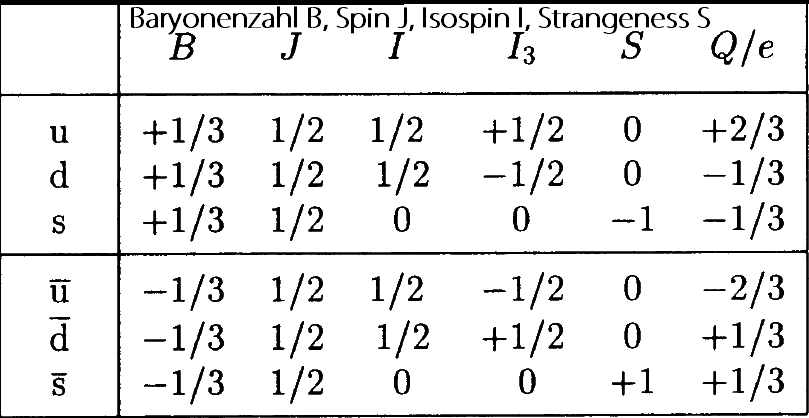
\includegraphics[width=.33\textwidth, height=100pt]{tab_quark}

\end{multicols*}
\end{document}